
\documentclass[border=10pt, 12pt]{standalone}
\usepackage[svgnames]{xcolor}
\usepackage{amsmath}
\usepackage{pgfplots}
\pgfplotsset{compat=newest}
\usepackage[sfdefault]{FiraSans}
\usepackage{FiraMono}
\renewcommand*\familydefault{\sfdefault}
\begin{document}
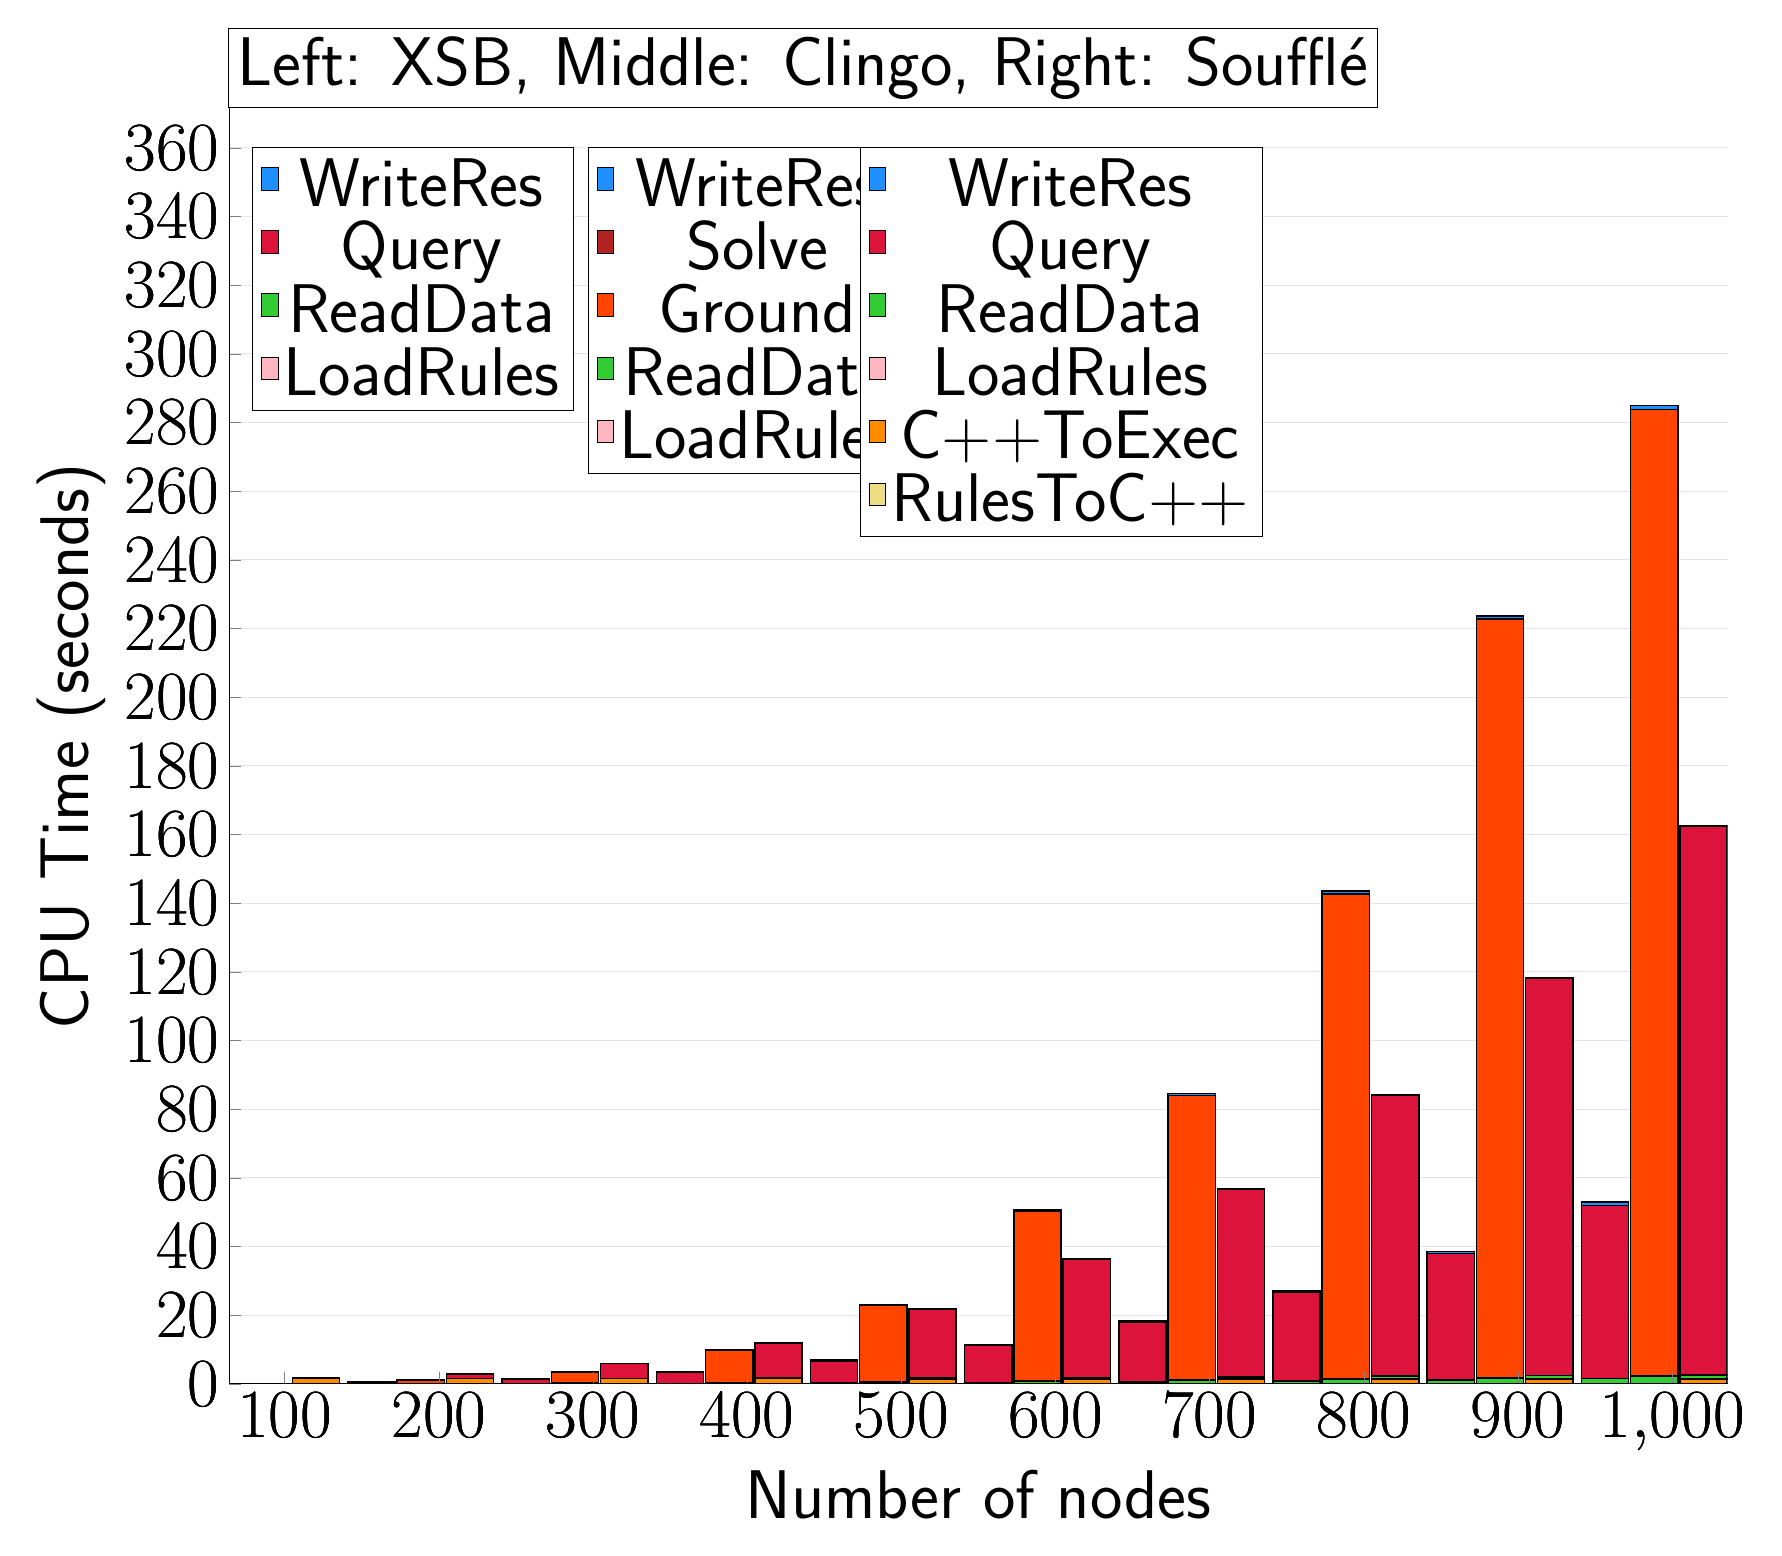
\begin{tikzpicture}
                        \begin{axis}[bar shift=-24.3pt, 
   ybar stacked,
   width=1.7\textwidth,
   bar width=0.6cm,
   ymajorgrids, tick align=inside,
   major grid style={draw=gray!20},
   xtick=data,
   ymin=0, ymax=371.479,
   axis x line*=bottom,
   axis y line*=left,
   enlarge x limits=0.04,
   legend style={
       at={(0.23, 0.97)},
       anchor=north east,
       legend columns=1,
       font=\Huge,
   },
   ylabel={CPU Time (seconds)},
   xlabel={Number of nodes},
   label style={font=\Huge},
   tick label style={font=\Huge},
]
\addlegendimage{fill=DodgerBlue, draw=black, line width=0.2pt}
\addlegendentry{WriteRes}
\addlegendimage{fill=Crimson, draw=black, line width=0.2pt}
\addlegendentry{Query}
\addlegendimage{fill=LimeGreen, draw=black, line width=0.2pt}
\addlegendentry{ReadData}
\addlegendimage{fill=LightPink, draw=black, line width=0.2pt}
\addlegendentry{LoadRules}
\addplot +[fill=LightPink, draw=black, line width=0.55pt] coordinates {
(100, 0.0005230000000000007)
(200, 0.0005109999999999997)
(300, 0.0005385999999999998)
(400, 0.0005469999999999996)
(500, 0.0005491999999999996)
(600, 0.0005465999999999997)
(700, 0.0005453999999999998)
(800, 0.0005455999999999996)
(900, 0.0005544000000000007)
(1000, 0.0005482000000000004)
};
\addplot +[fill=LimeGreen, draw=black, line width=0.55pt] coordinates {
(100, 0.0079926)
(200, 0.03419)
(300, 0.083649)
(400, 0.161444)
(500, 0.2689756)
(600, 0.4087468)
(700, 0.5962400000000001)
(800, 0.8283515999999999)
(900, 1.1241214000000002)
(1000, 1.5123718)
};
\addplot +[fill=Crimson, draw=black, line width=0.55pt] coordinates {
(100, 0.051374600000000006)
(200, 0.41375600000000007)
(300, 1.3822649999999999)
(400, 3.2706552)
(500, 6.3841808)
(600, 10.8373156)
(700, 17.2149548)
(800, 25.894326799999998)
(900, 36.7813652)
(1000, 50.468387199999995)
};
\addplot +[fill=DodgerBlue, draw=black, line width=0.55pt] coordinates {
(100, 0.0082572)
(200, 0.03457299999999998)
(300, 0.06898460000000002)
(400, 0.13466520000000007)
(500, 0.21245940000000002)
(600, 0.2701485999999999)
(700, 0.4217464000000007)
(800, 0.3708843999999992)
(900, 0.6451194000000001)
(1000, 1.0152350000000012)
};
\end{axis}

\begin{axis}[bar shift=-6.5pt, 
   ybar stacked,
   width=1.7\textwidth,
   bar width=0.6cm,
   ymajorgrids, tick align=inside,
   major grid style={draw=none},
   xtick=data,
   ymin=0, ymax=371.479,
   axis x line*=none,
   axis y line*=none,
   enlarge x limits=0.04,
   legend style={
       at={(0.454, 0.97)},
       anchor=north east,
       legend columns=1,
       font=\Huge,
   },
   label style={font=\Huge},
   tick label style={font=\Huge},
]
\addlegendimage{fill=DodgerBlue, draw=black, line width=0.2pt}
\addlegendentry{WriteRes}
\addlegendimage{fill=FireBrick, draw=black, line width=0.2pt}
\addlegendentry{Solve}
\addlegendimage{fill=OrangeRed, draw=black, line width=0.2pt}
\addlegendentry{Ground}
\addlegendimage{fill=LimeGreen, draw=black, line width=0.2pt}
\addlegendentry{ReadData}
\addlegendimage{fill=LightPink, draw=black, line width=0.2pt}
\addlegendentry{LoadRules}
\addplot +[fill=LightPink, draw=black, line width=0.55pt] coordinates {
(100, 0.0)
(200, 0.0)
(300, 0.0)
(400, 0.0)
(500, 0.0)
(600, 0.0)
(700, 0.0)
(800, 0.0)
(900, 0.0)
(1000, 0.0)
};
\addplot +[fill=LimeGreen, draw=black, line width=0.55pt] coordinates {
(100, 0.020000000000000018)
(200, 0.08000000000000002)
(300, 0.19)
(400, 0.344)
(500, 0.54)
(600, 0.782)
(700, 1.0740000000000003)
(800, 1.3979999999999997)
(900, 1.762)
(1000, 2.264)
};
\addplot +[fill=OrangeRed, draw=black, line width=0.55pt] coordinates {
(100, 0.11599999999999999)
(200, 0.9359999999999999)
(300, 3.1740000000000004)
(400, 9.294)
(500, 22.258000000000003)
(600, 49.39)
(700, 82.91)
(800, 141.31)
(900, 220.97600000000003)
(1000, 281.514)
};
\addplot +[fill=FireBrick, draw=black, line width=0.55pt] coordinates {
(100, 0.0)
(200, 0.0)
(300, 0.0060000000000000496)
(400, 0.010000000000000142)
(500, 0.012000000000000455)
(600, 0.026000000000000512)
(700, 0.030000000000001137)
(800, 0.046000000000003406)
(900, 0.054000000000000006)
(1000, 0.060000000000002274)
};
\addplot +[fill=DodgerBlue, draw=black, line width=0.55pt] coordinates {
(100, 0.01200000000000001)
(200, 0.050000000000000044)
(300, 0.09999999999999991)
(400, 0.18400000000000039)
(500, 0.29399999999999854)
(600, 0.4060000000000018)
(700, 0.5579999999999974)
(800, 0.7319999999999937)
(900, 0.9220000000000026)
(1000, 1.1340000000000063)
};
\end{axis}

\begin{axis}[bar shift=11.3pt, 
   ybar stacked,
   width=1.7\textwidth,
   bar width=0.6cm,
   ymajorgrids, tick align=inside,
   major grid style={draw=none},
   xtick=data,
   ymin=0, ymax=371.479,
   axis x line*=none,
   axis y line*=none,
   enlarge x limits=0.04,
   legend style={
       at={(0.69, 0.97)},
       anchor=north east,
       legend columns=1,
       font=\Huge,
   },
   label style={font=\Huge},
   tick label style={font=\Huge},
]
\addlegendimage{fill=DodgerBlue, draw=black, line width=0.2pt}
\addlegendentry{WriteRes}
\addlegendimage{fill=Crimson, draw=black, line width=0.2pt}
\addlegendentry{Query}
\addlegendimage{fill=LimeGreen, draw=black, line width=0.2pt}
\addlegendentry{ReadData}
\addlegendimage{fill=LightPink, draw=black, line width=0.2pt}
\addlegendentry{LoadRules}
\addlegendimage{fill=DarkOrange, draw=black, line width=0.2pt}
\addlegendentry{C++ToExec}
\addlegendimage{fill=LightGoldenrod, draw=black, line width=0.2pt}
\addlegendentry{RulesToC++}
\addplot +[fill=LightGoldenrod, draw=black, line width=0.55pt] coordinates {
(100, 0.010000000000000002)
(200, 0.008000000000000002)
(300, 0.0020000000000000005)
(400, 0.004000000000000001)
(500, 0.0)
(600, 0.0)
(700, 0.0)
(800, 0.0020000000000000005)
(900, 0.0)
(1000, 0.0)
};
\addplot +[fill=DarkOrange, draw=black, line width=0.55pt] coordinates {
(100, 1.478)
(200, 1.4780000000000002)
(300, 1.484)
(400, 1.482)
(500, 1.48)
(600, 1.474)
(700, 1.4759999999999998)
(800, 1.4739999999999998)
(900, 1.468)
(1000, 1.4680000000000002)
};
\addplot +[fill=LightPink, draw=black, line width=0.55pt] coordinates {
(100, 0.00012599999999999997)
(200, 0.00014319999999999998)
(300, 0.0001568)
(400, 0.00014680000000000002)
(500, 0.0001516)
(600, 0.00016199999999999998)
(700, 0.00016199999999999998)
(800, 0.0001752)
(900, 0.0001776)
(1000, 0.00016560000000000001)
};
\addplot +[fill=LimeGreen, draw=black, line width=0.55pt] coordinates {
(100, 0.0231698)
(200, 0.0680428)
(300, 0.123924)
(400, 0.20444279999999998)
(500, 0.3042548)
(600, 0.43476360000000003)
(700, 0.58579)
(800, 0.7591964)
(900, 0.9527090000000001)
(1000, 1.1774799999999999)
};
\addplot +[fill=Crimson, draw=black, line width=0.55pt] coordinates {
(100, 0.1734828)
(200, 1.288742)
(300, 4.2965919999999995)
(400, 10.239619999999999)
(500, 20.02356)
(600, 34.38988)
(700, 54.67282)
(800, 81.8471)
(900, 115.75139999999999)
(1000, 159.716)
};
\addplot +[fill=DodgerBlue, draw=black, line width=0.55pt] coordinates {
(100, 0.0023466)
(200, 0.008988600000000003)
(300, 0.019614600000000003)
(400, 0.0344806)
(500, 0.053383799999999995)
(600, 0.0766324)
(700, 0.104575)
(800, 0.1353092)
(900, 0.17125100000000001)
(1000, 0.2109734)
};
\end{axis}


\node[anchor=south, draw, fill=white] at (rel axis cs:0.42,1) {\Huge Left: XSB, Middle: Clingo, Right: Soufflé};
\end{tikzpicture}
\end{document}
                    